\begin{frame}{Approach}
\framesubtitle{Multihop Routing}

\begin{itemize}
    \item Implementation already exists
    \begin{itemize}
        \item RPL
    \end{itemize}
    \item No guaranty on
    \begin{itemize}
        \item Power efficiency
        \item Reliability
    \end{itemize}
    \item Lack of MAC protocol
\end{itemize}
\end{frame}

\begin{frame}{Approach}
\framesubtitle{Time Slotted Channel Hopping (TSCH)}

\begin{columns}
\begin{column}{0.5\textwidth}

Made for IEEE802.15.4 Phy

\begin{itemize}
  \item Time Division Multiplexing
  \begin{itemize}
    \item Power Efficient
    \item No collision
  \end{itemize}
  \only<2->{
  \item Frequency Division Multiplexing
  \begin{itemize}
    \item External interference resilience
    \item Concurrent transmission
  \end{itemize}
  }
\end{itemize}

\end{column}
\begin{column}{0.5\textwidth}

\begin{figure}[H]
\centering

  \resizebox{5cm}{4cm}{%
  \begin{tikzpicture}[
    asn/.style={black!70, minimum size=1cm},
    timeslot/.style={draw, rectangle, minimum size=1cm},
    arr/.style={help lines,black!70,<->},
    desc/.style={black!70},
  ]
    \only<2->{
    \foreach [evaluate={\ts=int(mod(\i, 4))}] \i in {0,...,7} {
    \node (ts3\i) [timeslot] at (\i, 3) {};
    }
    \foreach [evaluate={\ts=int(mod(\i, 4))}] \i in {0,...,7} {
    \node (ts2\i) [timeslot] at (\i, 2) {};
    }
    }
    \foreach [evaluate={\ts=int(mod(\i, 4))}] \i in {0,...,7} {
    \node (ts1\i) [timeslot] at (\i, 1) {};
    }
    \foreach [evaluate={\ts=int(mod(\i, 4))}] \i in {0,...,7} {
    \node (ts\i) [asn] at (\i, 0) {$TS_{\ts}$};
    }

    \only<2->{
    \node (choff3) [black!70] at (-1.5, 3) {$Ch_{off} 2$};
    \node (choff2) [black!70] at (-1.5, 2) {$Ch_{off} 1$};
    \node (choff1) [black!70] at (-1.5, 1) {$Ch_{off} 0$};
    }

    \begin{scope}[on background layer]
    \only<2->{
    \fill[green!50] (ts22.south west) rectangle (ts22.north east);
    \fill[green!50] (ts36.south west) rectangle (ts36.north east);

    \fill[orange!50] (ts30.south west) rectangle (ts30.north east);
    \fill[orange!50] (ts14.south west) rectangle (ts14.north east);

    \fill[blue!50] (ts24.south west) rectangle (ts24.north east);
    }

    \fill[blue!50] (ts10.south west) rectangle (ts10.north east);
    \end{scope}

    \only<2->{
        \draw[ultra thick]
        (ts10.south west) rectangle (ts33.north east)
        (ts14.south west) rectangle (ts37.north east);
    }
    \only<1>{
        \draw[ultra thick]
        (ts10.south west) rectangle (ts13.north east)
        (ts14.south west) rectangle (ts17.north east);
    }

    \draw[arr,->]
    ([yshift=-10pt]ts0.south west) -- node[fill=white] {$time$} ([yshift=-10pt]{ts7.south east});

  \begin{scope}[xshift=2.5cm,yshift=-3cm,->,>=stealth',shorten >=1pt,auto,node distance=2.5cm]
    \tikzstyle{every state}=[thick,draw=gray!50,fill=gray!20,draw=none,text=black]

    \node[state]         (A) [] {A};
    \node[state]         (B) [below of=A]       {B};
    \node[state]         (C) [right of=B]       {C};

    \only<2-> {
      \path (A) edge [bend left,draw=orange!50] node[draw=orange!50] {$TS_1$} (C)
          (B) edge [bend left,draw=blue!50] node[draw=blue!50] {$TS_1$} (A)
          (C) edge [bend left,draw=green!50] node[above right,draw=green!50] {$TS_3$} (A);
    }
    \only<1> {
      \path (B) edge [bend left,draw=blue!50] node[draw=blue!50] {$TS_1$} (A);
    }
  \end{scope}
\end{tikzpicture}
}
\caption{TSCH Schedule\label{fig:customsched}}
\end{figure}
\end{column}
\end{columns}
\end{frame}

\begin{frame}{Approach}
\framesubtitle{TSCH - Time Slots}

\resizebox{11.2cm}{3.8cm}{%
\begin{tikzpicture}[
  timeslot/.style={draw, rectangle, minimum size=1cm},
  description/.style={draw, rectangle, minimum size=1cm},
  arr/.style={help lines,black!70,<->},
]

\foreach [evaluate={\ts=int(mod(\i, 4))}] \i in {0,...,7} {
  \node (ts\i) [timeslot] at (\i, 0) {$TS_{\ts}$};
}
\node (ts8) [minimum height=1cm, minimum width=2cm, black!70] at (8.5, 0) {\ldots};

\draw[help lines, black!70]
  (ts8.north west) -- (ts8.north east) node[fill=white, black!70] {$\ldots$};
\draw[help lines, black!70]
  (ts8.south west) -- (ts8.south east) node[fill=white, black!70] {$\ldots$};

\draw[ultra thick] 
  (ts0.south west) rectangle (ts3.north east)
  (ts4.south west) rectangle (ts7.north east);

\begin{scope}[xshift=-1.2cm,yshift=-2.5cm,inner sep=0pt, outer sep=0pt]
  \node (desc) [draw,rectangle,fit={(0,0) (14,1)}, label=left:{Transmitter~}] {};
  \node (desc1) [description, fill=orange!20, fit={(3,0) (6,1)}, label=center:{data}] {};
  \node (desc0) [description, fill=gray!20, fit={(1,0) (3,1)}, label=center:{tx\_offset}] {};
  \only<2->{
  \node (descsync1) [description, fill=blue!20, fit={(6.7,0) (7,1)}] {};
  \node (descsync2) [description, fill=blue!20, fit={(9.5,0) (9.8,1)}] {};
  \node (desc2) [description, fill=gray!20, fit={(7,0) (9.5,1)}, label=center:{rx\_ack\_delay}] {};
  \draw[arr,<->]
      ([yshift=-10pt]descsync1.south west) -- node[fill=white] {$guard$} ([yshift=-10pt]{descsync2.south east});
  }
\end{scope}

\draw[help lines, black!70,-]
  ([yshift=0pt]ts4.south west) -- 
  ([yshift=0pt]{desc.north west});
\draw[help lines, black!70,-]
  ([yshift=0pt]ts4.south east) -- 
  ([yshift=0pt]{desc.north east});

\begin{scope}[xshift=-1.2cm,yshift=-4.5cm,inner sep=0pt, outer sep=0pt]
  \node (ddesc) [draw,rectangle,fit={(0,0) (14,1)}, label=left:{Receiver~}] {};
  \node (ddescsync1) [description, fill=blue!20, fit={(0.7,0) (1,1)}] {};
  \node (ddescsync2) [description, fill=blue!20, fit={(3,0) (3.3,1)}] {};
  \node (ddesc0) [description, fill=gray!20, fit={(1,0) (3,1)}, label=center:{rx\_offset}] {};
  \draw[arr,<->]
      ([yshift=-10pt]ddescsync1.south west) -- node[fill=white] {$guard$} ([yshift=-10pt]{ddescsync2.south east});
  \only<2->{
  \node (ddesc2) [description, fill=gray!20, fit={(7,0) (9.5,1)}, label=center:{tx\_ack\_delay}] {};
  \node (ddesc3) [description, fill=orange!20, fit={(9.5,0) (12,1)}, label=center:{ack}] {};
  }
\end{scope}

\draw[help lines, black!70,-]
    (desc.south west) -- ({ddesc.north west});
\draw[help lines, black!70,-]
    (desc.south east) -- ({ddesc.north east});
\end{tikzpicture}
}
\end{frame}

\begin{frame}{Approach}
\framesubtitle{TSCH - Channel Hopping}

\begin{columns}
\begin{column}{0.5\textwidth}
  \resizebox{5cm}{2.5cm}{%
  \begin{tikzpicture}[
    asn/.style={black!70, minimum size=1cm},
    timeslot/.style={draw, rectangle, minimum size=1cm},
    arr/.style={help lines,black!70,<->},
    desc/.style={black!70},
  ]
    \foreach [evaluate={\ts=int(mod(\i, 4))}] \i in {0,...,7} {
    \node (ts3\i) [timeslot] at (\i, 3) {};
    }
    \foreach [evaluate={\ts=int(mod(\i, 4))}] \i in {0,...,7} {
    \node (ts2\i) [timeslot] at (\i, 2) {};
    }
    \foreach [evaluate={\ts=int(mod(\i, 4))}] \i in {0,...,7} {
    \node (ts1\i) [timeslot] at (\i, 1) {};
    }
    \foreach [evaluate={\ts=int(mod(\i, 4))}] \i in {0,...,7} {
    \node (ts\i) [asn] at (\i, 0) {$TS_{\ts}$};
    }

    \node (choff3) [black!70] at (-1.5, 3) {$Ch_{off} 2$};
    \node (choff2) [black!70] at (-1.5, 2) {$Ch_{off} 1$};
    \node (choff1) [black!70] at (-1.5, 1) {$Ch_{off} 0$};

    \begin{scope}[on background layer]
    \fill[green!50] (ts22.south west) rectangle (ts22.north east);
    \fill[green!50] (ts36.south west) rectangle (ts36.north east);

    \fill[orange!50] (ts30.south west) rectangle (ts30.north east);
    \fill[orange!50] (ts14.south west) rectangle (ts14.north east);

    \fill[blue!50] (ts24.south west) rectangle (ts24.north east);
    \fill[blue!50] (ts10.south west) rectangle (ts10.north east);
    \end{scope}

    \draw[ultra thick]
        (ts10.south west) rectangle (ts33.north east)
        (ts14.south west) rectangle (ts37.north east);
    \draw[arr,->] ([yshift=-10pt]ts0.south west) -- node[fill=white] {$time$} ([yshift=-10pt]{ts7.south east});
\end{tikzpicture}
}
\end{column}
\begin{column}{0.5\textwidth}

\resizebox{5.5cm}{5cm}{%
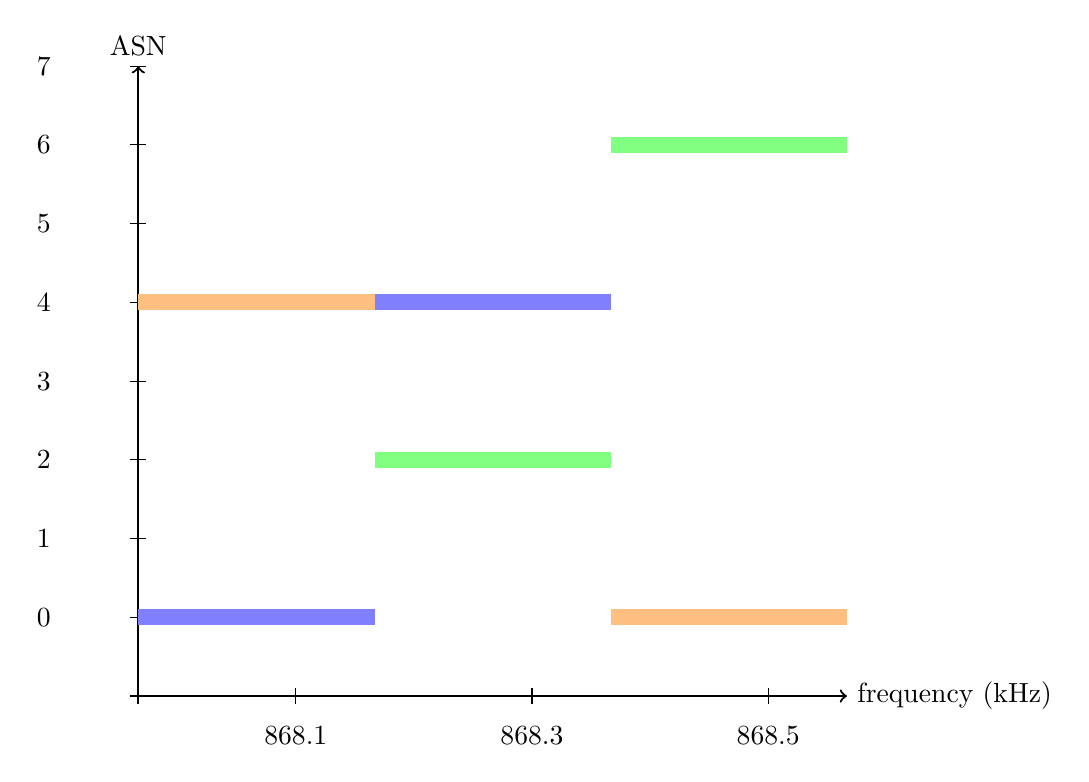
\begin{tikzpicture}
  \draw[->,thick] (-0.1,0)--(9,0) node[right]{frequency (kHz)};
  \draw[->,thick] (0,-0.1)--(0,8) node[above]{ASN};
  \node[] at (2, -0.5) {868.1};
  \draw[] (2,-0.1)--(2,0.1);
  \node[] at (5, -0.5) {868.3};
  \draw[] (5,-0.1)--(5,0.1);
  \node[] at (8, -0.5) {868.5};
  \draw[] (8,-0.1)--(8,0.1);

  \node[] at (-1.2, 1) {0};
  \draw[] (-0.1,1)--(0.1,1);
  \node[] at (-1.2, 2) {1};
  \draw[] (-0.1,2)--(0.1,2);
  \node[] at (-1.2, 3) {2};
  \draw[] (-0.1,3)--(0.1,3);
  \node[] at (-1.2, 4) {3};
  \draw[] (-0.1,4)--(0.1,4);
  \node[] at (-1.2, 5) {4};
  \draw[] (-0.1,5)--(0.1,5);
  \node[] at (-1.2, 6) {5};
  \draw[] (-0.1,6)--(0.1,6);
  \node[] at (-1.2, 7) {6};
  \draw[] (-0.1,7)--(0.1,7);
  \node[] at (-1.2, 8) {7};
  \draw[] (-0.1,8)--(0.1,8);

  \fill[blue!50] (0,0.9) rectangle (3,1.1);
  \fill[orange!50] (6,0.9) rectangle (9,1.1);
  \fill[green!50] (3,2.9) rectangle (6,3.1);

  \fill[blue!50] (3,4.9) rectangle (6,5.1);
  \fill[orange!50] (0,4.9) rectangle (3,5.1);
  \fill[green!50] (6,6.9) rectangle (9,7.1);
\end{tikzpicture}
}


\end{column}
\end{columns}

\end{frame}

\begin{frame}{Approach}
\framesubtitle{Porting TSCH}
\begin{itemize}
  \item LoRa multi-hop network
  \begin{itemize}
    \item Long range
    \item Power efficient
    \item Reliable
  \end{itemize}
  \item Contiki as starting point
  \item Using RPL
  \item Porting TSCH
  \begin{itemize}
    \item No implementation for LoRa
  \end{itemize}
  \item Radio driver for LoRa
\end{itemize}
\end{frame}
